\documentclass[10pt,conference,letterpaper]{IEEEtran}
\usepackage{graphicx}
\usepackage{subfigure}
\begin{document}
\section{experiment}

EARN is evaluated on a 5-node cluster on Amazon EC2, one as master and four as worker. Each node is of m4.2xlarge type with 8 cores and 32GB of memory. 20GB of memory is used for cache in worker nodes, which summarized to 80GB of cache in total.

We measured the performance of EARN under different circumstances in comparison to other different cache eviction strategies including LRU, LFU and MAXMIN.
One experiment is composed of scanning three files, which is denoted as FILE-1, FILE-2 and FILE-3.
There are three frequency patterns, meaning ROUND, ONE and TWO ass described below.
\begin{itemize}
\item ROUND: Three files are accessed in the same frequency.
\item ONE: One of the three files is accessed more frequently.
\item TWO: Two of the three files are accessed more frequently.
\end{itemize}
EARN uses the window size of 1000GB in default.

Fig.~\ref{fig:time_444} shows the average processing time of different strategies in different frequency patterns. Each file is 40GB in size. It can be seen that EARN is the fastest of all.
Fig.~\ref{fig:time_741} shows similar results where files are 70GB, 40GB and 10GB in size respectively.

More specifically, we analyzed the distribution of block accessing. As shown in Fig.~\ref{fig:block_count}, EARN has the largest number of blocks accessed in local or remote memory. It means that EARN has the highest memory efficiency compared to other strategies. This is also the reason EARN strategy is the fastest.

As we can see in the time figures, MAXMIN is close in time to our EARN strategy. Yet essentially, MAXMIN helps maintain the same amount of memory for all files or users, which can be a problem when some files stop been accessed or some users become inactive.
To illustrate this, we simulated a scenario where first all three files are accessed in the same frequency and later one or two files stops been accessed.
Fig.~\ref{fig:3-1} shows changes in amount of in-memory data after FILE-3 is not accessed. The X-axis is the number of experiments, which can be viewd as the dimension of time. 
Apparently, the remaining active files gains more memory resource with time going in EARN strategy, while FILE-3 still holds nearly 1/3 of total memory even it's not accessed. That is quite a waste of limited memory resource.

Fig.~\ref{fig:3-2} shows similar results when both FILE-2 and FILE-3 are not accessed any more. The gain in memory of FILE-1 is more remarkable.

Finally, we also analyzed the impact of window size. As shown in Fig.~\ref{fig:time_windowsize}, when windown size is too small, the time performance will degrade.

\begin{figure}[!htbp]
\centering
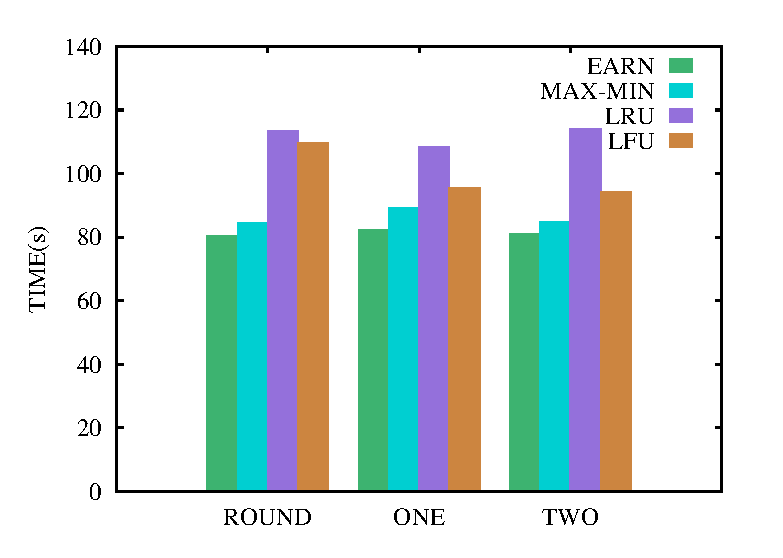
\includegraphics[scale=0.4]{figures/scan444_time.eps}
\caption{Access Time. Three files are equal in size (40GB).}
\label{fig:time_444}
\end{figure}

\begin{figure}[!htbp]
\centering
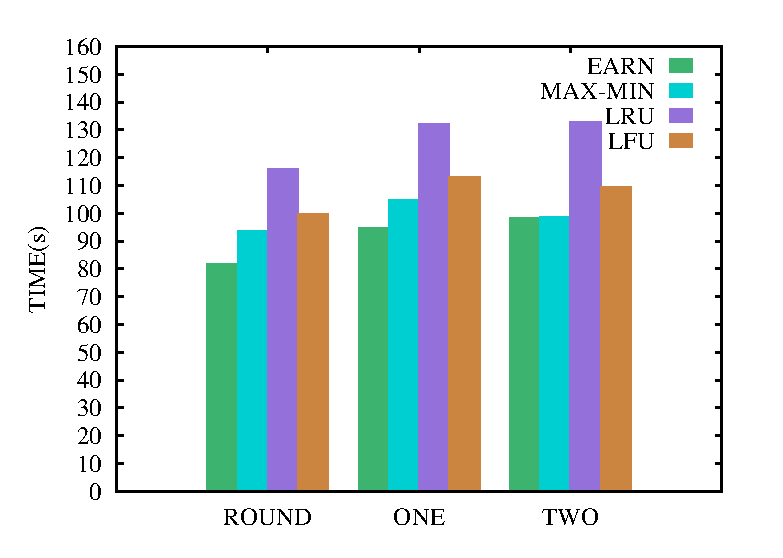
\includegraphics[scale=0.4]{figures/scan741_time.eps}
\caption{Access Time. The size of files is 70GB, 40GB and 10GB respectively.}
\label{fig:time_741}
\end{figure}


\begin{figure}[!htbp]
    \subfigure[ROUND]{
    		\begin{minipage}[b]{0.25\linewidth}
    		\centering
    		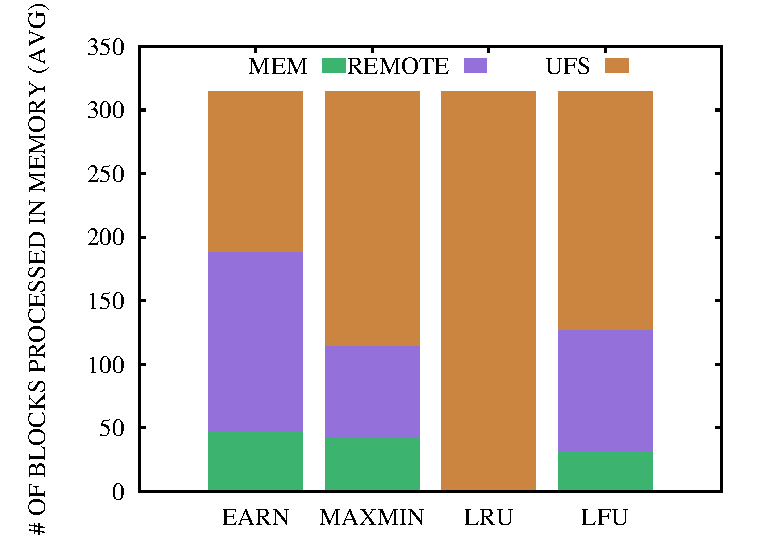
\includegraphics[scale=0.2]{figures/block_count_avg_round.eps}
    		\end{minipage}
    }
    \subfigure[ONE]{
        \begin{minipage}[b]{0.25\linewidth}
        \centering
        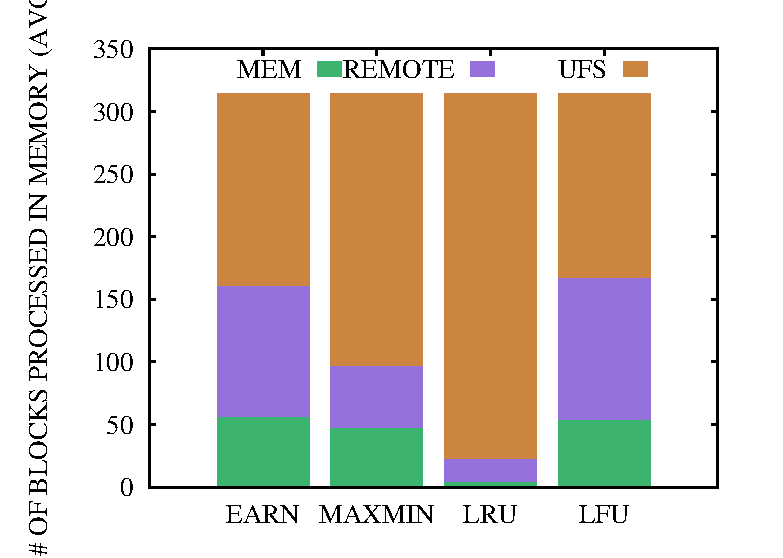
\includegraphics[scale=0.2]{figures/block_count_avg_one.eps}
        \end{minipage}
    }
    \subfigure[TWO]{
        \begin{minipage}[b]{0.25\linewidth}
        \centering
        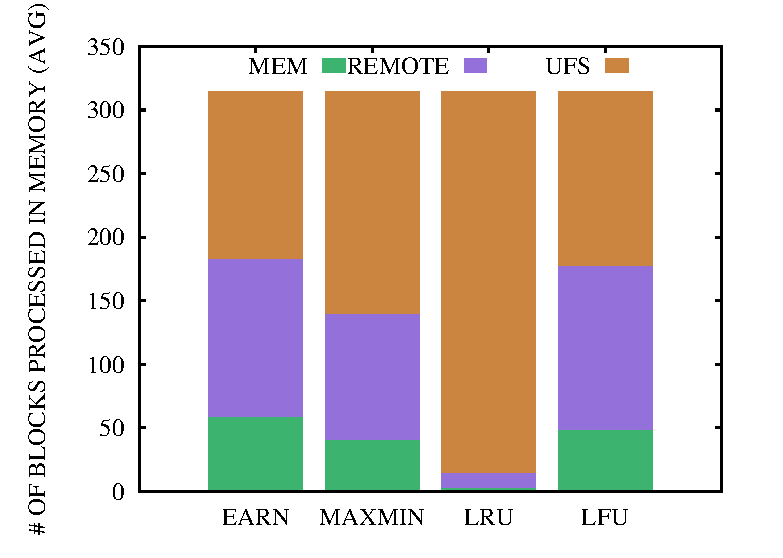
\includegraphics[scale=0.2]{figures/block_count_avg_two.eps}
        \end{minipage}
    }
    \caption{Distribution of blocks accessed in memory, remote memory and under file system.}
    \label{fig:block_count}
\end{figure}


\begin{figure}[!htbp]
    \subfigure[EARN]{
    		\begin{minipage}[b]{0.45\linewidth}
    		\centering
    		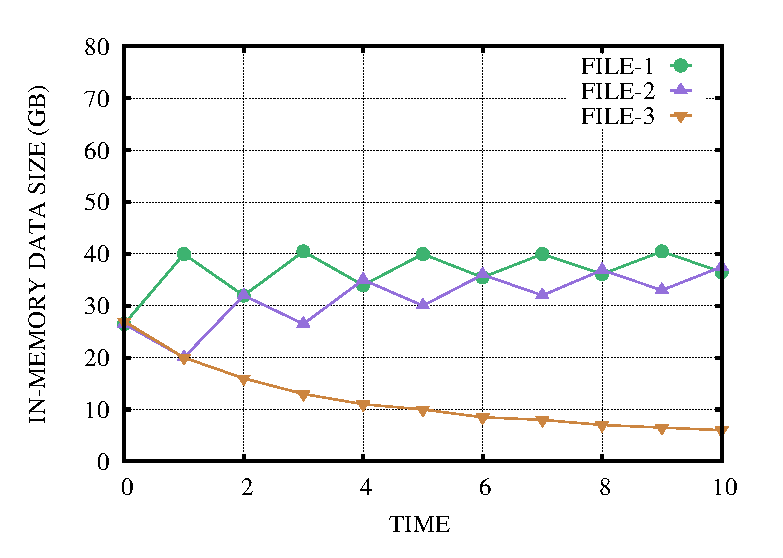
\includegraphics[scale=0.34]{figures/3-1-earn-1000-ds.eps}
    		\end{minipage}
    }
    \subfigure[MAXMIN]{
        \begin{minipage}[b]{0.45\linewidth}
        \centering
        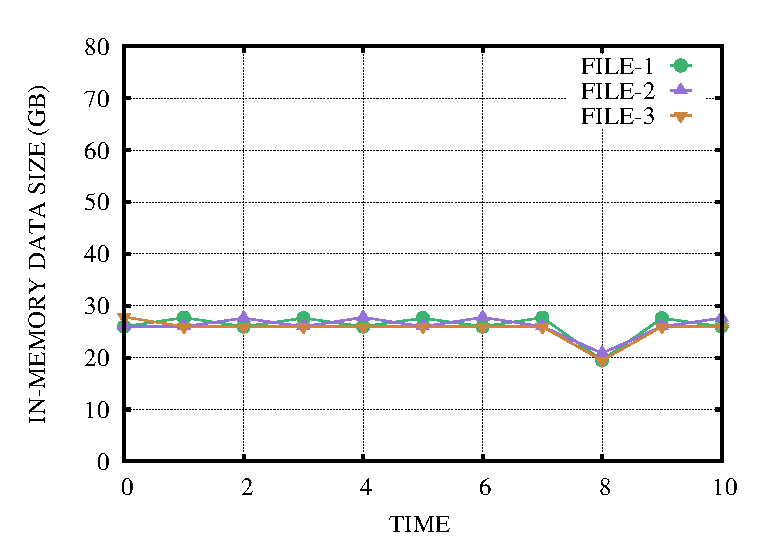
\includegraphics[scale=0.34]{figures/3-1-maxmin-1000-ds.eps}
        \end{minipage}
    }
    \caption{In-memory data size of each file after File-3 stops been visited.}
    \label{fig:3-1}
\end{figure}


\begin{figure}[!htbp]
    \subfigure[EARN]{
    		\begin{minipage}[b]{0.45\linewidth}
    		\centering
    		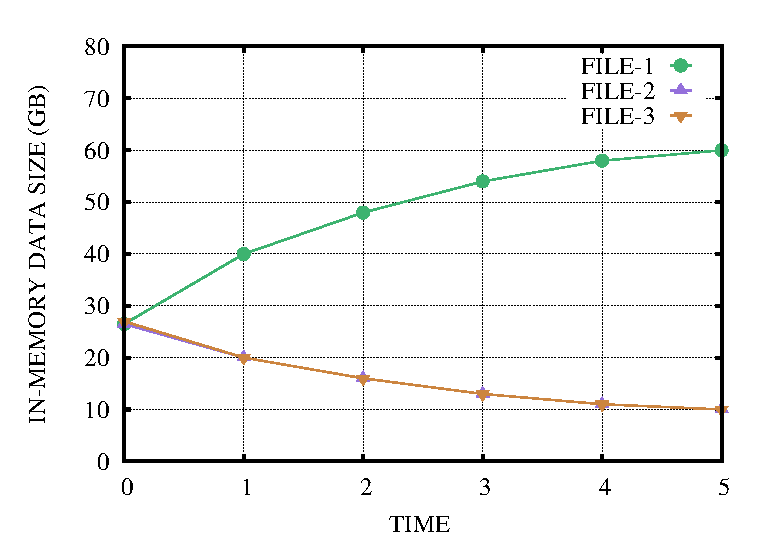
\includegraphics[scale=0.34]{figures/3-2-earn-1000-ds.eps}
    		\end{minipage}
    }
    \subfigure[MAXMIN]{
        \begin{minipage}[b]{0.45\linewidth}
        \centering
        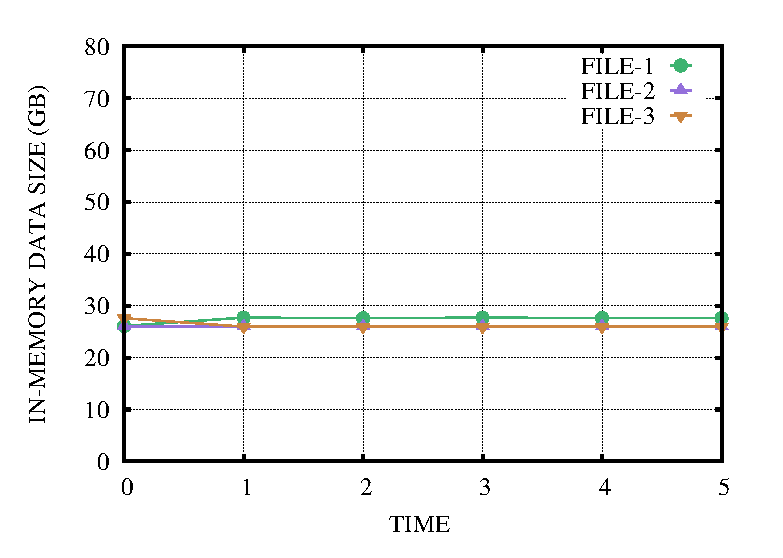
\includegraphics[scale=0.34]{figures/3-2-maxmin-1000-ds.eps}
        \end{minipage}
    }
    \caption{In-memory data size of each file after File-3 and File-2 stop been visited.}
    \label{fig:3-2}
\end{figure}


\begin{figure}[!htbp]
\centering
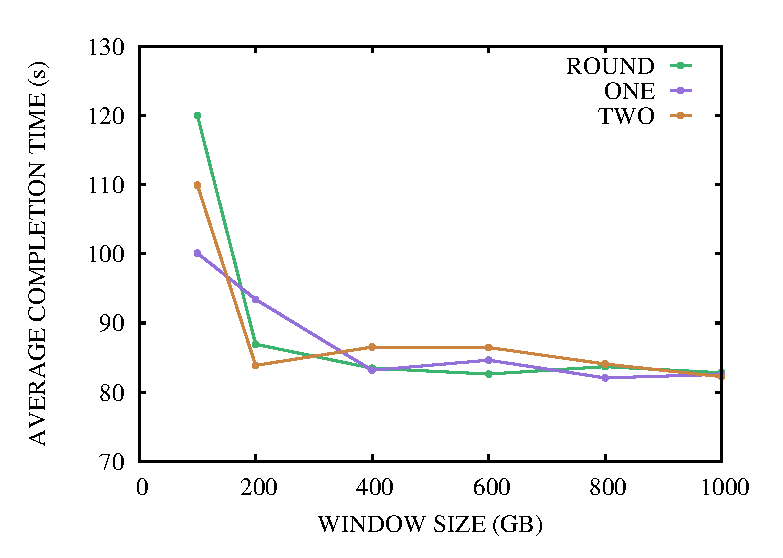
\includegraphics[scale=0.4]{figures/window_size_time.eps}
\caption{Access Time. Each with different window size.}
\label{fig:time_windowsize}
\end{figure}

\end{document}